
% :::::: IV - Proposed Solution ::::::::::::::::::
\section{Proposed Solution}
\label{Proposed Solution}
% Here we provide a detailed description about our {\em W} system. We start by describing how to ...in~\ref{module1} then we proceed to show how module....

\begin {figure}[t]
\centering
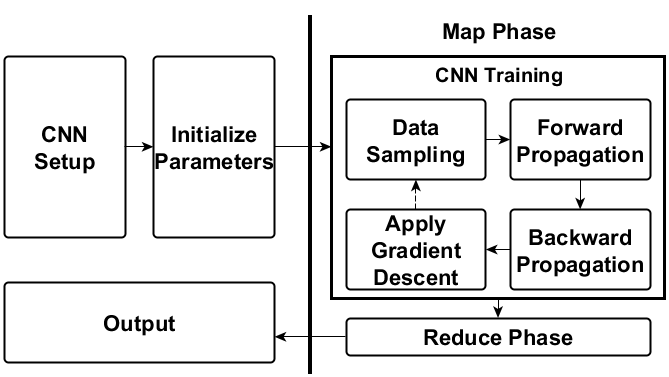
\includegraphics[width=0.99\columnwidth]{Paper_Fig2_CNN-DistComputing.png} % Was pic14.png
%\vspace{-10pt}
\caption{Solution Architecture for CNN with Distributed Computing}
\label{Solution Architecture for CNN with Distributed Computing}
%\vspace{-10pt}
\end {figure}

In this section we discuss our proposed solution along with various aspects that contribute to the solution. First the solution architecture is discussed followed by our main idea (our proposed solution). Next our algorithm is presented. In the next two sections we explain convolutional layers and pooling as well as backpropagation which play central roles in our solution and algorithm. We finally present a brief analysis on cost and correctness.
 
\subsection{Solution Architecture}
First, we implement the naive CNN algorithm with single process, as it is originally used. The CNN part is implemented by Python with Tensorflow library. Tensorflow is an open source Python library developed by Google, which helps users to implement the deep learning algorithms in a more efficient way. CNN training consists of data sampling followed by forward propagation and then back propagation. Weights are adjusted via gradient descent. 
Second, we add the distributed computing to the naive model. This process is also implemented by Python. The reason why we try to use the same programming language is to facilitate the calling and communication process between different languages which in turn will not require extra time. Using different programming languages may require extra computation time, which is a disadvantage. With the distributed computing model, CNN training is distributed across machines in the Map Phase; the weights are then combined to formulate the final model in the Reduce Phase. The final output (result) is then produced. 


\subsection{Main Idea}
\label{MainIdea}
The naive CNN model (see Fig. \ref{Naive Training Framework} is a simple non-distributed model which acts as a baseline that we use to compare our proposed distributed computing model.
% describe the main idea
Based on the naive CNN model, we can already reach a reasonable accuracy. However, the training process costs much time and in this module we want to reduce the time consumption by distributed computing. Thus we implemented this method to map different parts of the input dataset into different machines and then do the training process simultaneously. After that we collect all the weight matrices and combine them to formulate a final model. (See Fig. \ref{Distributed Training Framework})

\begin {figure}[t]
\centering
% \includegraphics[width=7cm]{pic15.png}
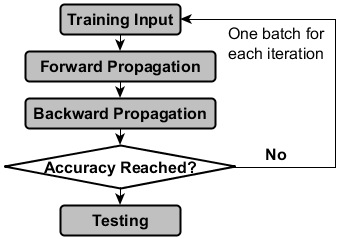
\includegraphics[width=0.7\columnwidth]{Paper_Fig5_NaiveTrainingFramework.png} % Was Fig7NaiveTrFrWk.png
\caption{Naive Training Framework}
\label{Naive Training Framework}
%\vspace{-10pt}
\end {figure}


\subsection{Algorithm}
% If exists, Provide the pseudo code of your first algorithm behind this module
% Line-by-Line or block-by-block explanation for the pseudo code with reference to the line or the block in the algorithm.
Unlike the baseline naive CNN model mentioned in the previous section, in this strategy, distributed computing is injected directly into the convolutional neural network. Due to the highly complex structure of the CNN model, a distributed computing method is implemented to handle the large amount of computation involved. 

In the distribution block, each machine would be assigned to one batch of input, and they will simultaneously execute the training process individually, which has already been implemented in the first module. In other words, each machine also goes through the convolutional process, pooling process, and the fully-connected process. After that the back propagation is used to update the parameters individually based on the same initial weights, which is explained by Fig. \ref{Naive Training Framework}. 

In the combination block, we collect all the trained neural network model, and combine their parameters together with vector operations. To be more specific, the matrices used to store the weights are collected to one machine and then the corresponding values are added based on the matrix operation. Then we obtain the final model.

Finally, we do the testing process with the testing dataset to see if they are correctly combined and analyze the time consumption in the experiment section.
%%%%%%%%%%%%%%%%%%%%%%%%%%%%%%%%%%%
\begin{algorithm}[t]
\caption{Distributed Computing CNN Training Algorithm}
\label{alg1}  % \label{alg2}
\begin{algorithmic}[1]
\begin{codebox}
%\label{alg1}
%\Procname{$\proc{Distributed Computing CNN Training Algorithm}$}
\li $Get$ $path()$
\li $Input \gets image$
\li $Initialize$ $neural$ $network$ $weights$
\li \For $each$ $input$ $batch:$
\li      \hspace*{1cm}$Assign$ $it$ $to$ $one$ $machine$ 
\End
\li \For $each$ $machine :$
\li      \hspace*{1cm}$Get$ $initial$ $weights$
\li      \hspace*{1cm}$Training$ $Process$
\li      \hspace*{1cm}\For $each$ $training$ $iteration:$
\li      \hspace*{2cm}$Read$ $One$ $Batch$ $Input$
\li      \hspace*{2cm}$Start$ $training$ $process :$
\li      \hspace*{3cm}$Forward$ $propapagtion:$
\li      \hspace*{3cm}$Convolution$ $process$
\li      \hspace*{3cm}$Sampling$ $process$
\li      \hspace*{3cm}$Fully$ $connected$ $process$
\li      \hspace*{2cm}$Backward$ $propapagtion:$
\li         \hspace*{3cm}$Calculate$ $gradient$ $descent$
\li         \hspace*{3cm}$Weight$ $update$
\li         \hspace*{2cm}$offset \gets backward$ $propagation()$ \End
\li $Collect$ $all$ $weight$ $matrices$ $to$ $main$ $machine$
\li $Combine$ $the$ $corresponding$ $weights$
\li $Final$ $parameters \gets combined$ $parameters$
\li $Testing$ $Process$
\li \For $each$ $testing$ $iteration:$
\li     \Do $read$ $one$ $image$
\li         $execute$ $CNN$ $model$
\li 		$output \gets recognized$ $digit$
\End
\end{codebox}
\end{algorithmic}
\end{algorithm}
%%%%%%%%%%%%%%%%%%%%%%%%%%%%%%%%%%%


\subsection{Convolutional Layers and Pooling}
CNN is a special case of neural network. Compared to normal neutral network it has two specialities. The first is some layers are not fully connected to its previous or next layer. The second is some clusters of nodes share common weights. These two specialities are generated because two special layers exist in CNN, which are called convolutional layer and pooling layer.

Convolution is an important operation for image processing. Applying convolution with a convolutional kernel is essentially a filter process. The basic math presentation for convolution is:
\begin{equation}
f(x,y)\ast g(x,y)=\sum_{s=-a}^{a} \sum_{t=-b}^{b} w(s,t)f(x-s,y-t)
\label{Eq1Conv}
\end{equation}
$I=f(x,y)$ is an input image, $f(x,y)$ is the gray value for the pixel at row $x$ and column $y$. $w(x,y)$ is called convolutional kernel, while $a$ and $b$ define the size of $w(x,y)$.

We can see from Eq \eqref{Eq1Conv} that convolution is essentially a weighted summary operation. The kernel slides on the image, aligns its center to each pixel and calculates the weighted average for covered region as the response of this pixel.

The reason why such convolutional layers are introduced into neutral network is that, human being's visual recognizing process is hierarchical. Lower layers extract some edge features while higher layers capture shape and motion information. From low layer to high layer, extracted features become more and more abstract. Since in computer vision, image feature extraction relies on convolution, we add two or three convolutional layers to simulate this procedure and extract different kinds of features from input images. Each convolutional layer is an image convolution of the previous layer, where the weights specify the convolution filter.

Another advantage of convolutional layer is weight-sharing. Suppose the size of input image is $13\times 13$, which means the input layer has 169 neutrons. For fully connected layer, with only 20 neutrons, we have to set $(169+1)\times 20$ weights. Convolutional layers reduce the number of weights dramatically. If we use $5\times 5$ kernel, and generate 6 feature maps for this convolutional layer, we only have to set $(5\times 5+1)\times 6$ weights.

If we denote the k-th feature map at a given layer as $h^k$, whose filters are determined by the weights $W^k$ and bias $b_k$, then the feature map $h^k$ is obtained as follows ($F$ denotes a non-linear active function):
\begin{equation}
h_{ij}^k=F((W^k\ast x)_{ij}+b_k)
\end{equation}
$k\in [0,k]$ means we have $k$ feature maps as output as well as $k$ kernels for convolution. 

After each convolutional layer, there may be a pooling layer. This is because using all extracted features from the previous convolutional layer would be quite challenging. The aim is to reduce such a large number of neutrons that would increase computation complexity to unacceptable levels. Reducing the number of features would also reduce the possibility of overfitting.

To solve such problems, statistics from the feature maps are collected, and make each feature represent a local region instead of a single pixel. This process is called down-pooling. Generally, there are two main strategies for pooling that are used: max-pooling and mean-pooling. Both of them first partition the output feature maps of previous convolutional layer (i.e. the input into the current pooling layer) into non-overlapping rectangles. For each sub-region, max-pooling takes the maximum value as the output and mean-pooling takes the average value as the output. By doing this, a single output is produced for that block which reduces the difficulty of the problem.
%%%%%%%%%%%%%%%%%%%%%%%%%%%%%%%%%%%
\begin {figure}[t]
\centering
% \includegraphics[width=8cm]{pic16.png}
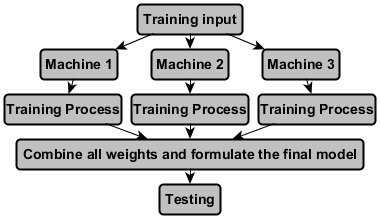
\includegraphics[width=0.90\columnwidth]{Fig8DistTrFrWk.png}
%\vspace{-10pt}
\caption{Distributed Training Framework}
\label{Distributed Training Framework}
%\vspace{-10pt}
\end {figure}
%%%%%%%%%%%%%%%%%%%%%%%%%%%%%%%%%%%
\subsection{Back propagation for CNN}
Back propagation (BP) for fully connected layers, such as in a neural network, is straightforward. However, in this algorithm, with the presence of convolutional and pooling layers, the situation is slightly different [5]. Let $\delta^{l+1}$ be the error term for the $(l+1)$-st layer in the network with a cost function $J(W,b;x,y)$ where $(W,b)$ are the parameters and $(x,y)$ are the training data and label pairs. If the $l$-th layer is a pooling layer then the error is propagated through as:
\begin{equation}
\delta_k^{(l)}=upsample(\delta_k^{(l+1)})
\label{EqUpSample}
\end{equation}
Eq \eqref{EqUpSample} illustrates the process of reverse max pooling. The upsample operation propagates the error through the pooling layer by putting the error from layer $l+1$ to layer $l$. During forward pooling, we record which pixel is the local maximum. During reverse pooling, we put the error back to that local maximum position and set all the other positions as 0.

If the $l$-th layer is a convolutional layer then the error is propagated through as:
\begin{equation}
\delta_k^{(l)}=((W_{(k)}^{l})^{\rm T}\delta_k^{(l+1)})\cdot f'(z_k^l)
\end{equation}
The main difference from BP in fully connected layer is, we need to choose the correct weight matrix according to which convolution kernel generates the node with $\delta_k^{(l+1)}$ error.

Once we get the error term for each node in the CNN, we can take a step further to calculate the gradient w.r.t to the weights and bias. we rely on the border handling convolution operation again and flip the error matrix $\delta_k^l$ the same way we flip the filters in the convolutional layer.
\begin{equation}
\begin{split}
\nabla_{W_k^{(l)}}J(W,b;x,y)=\sum_{i=1}^m(a_i^{(l)})\ast\\ rot90(\delta_k^{(l+1)},2), \nabla_{b_k^{(l)}}J(W,b;x,y) =\\ \sum_{a,b}^{i=1}(\delta_k^{(l+1)})_{a,b}.
\end{split}
\end{equation}

Where $a^{(l)}$ is the input to the $l$-th layer, and $a^{(1)}$ is the input image. The operation $(a^{(l)}_i)\ast\delta^(l+1)_k$ is the ``valid'' convolution between $i$-th input in the $l$-th layer and the error w.r.t. the $k$-th filter.

\subsection{Expanding Data Sets through Elastic Distortions}
Given a classification task, one may apply transformations to generate additional data and let the learning algorithm infer the transformation invariance. [13] states that by introducing elastic distortion to original data set, they get better result than approach with simple affine transformation. Following their strategy, we integrate this part into our project, to justify its validation and improve our final result.

For every pixel in the original image, we compute a new target location with respect to the original location. The new target location, at position $(x,y)$ is given with respect to the previous position. For instance, if $D^x_{(x,y)}=1$ and $D^y_{(x,y)}=0.5$, it means the new location of $(x,y)$ is shifted by 1 to the right and 0.5 to the bottom. If the displacement field is $D^x_{(x,y)}=\alpha x$ and $D^y_{(x,y)}=\alpha y$, that means the displacement is scaled by $\alpha$ from the origin location.

As initialization, we randomly generate values for vertical and horizontal displacement. That is, we first set $D^x_{(x,y)}=rand(-1,1)$ and $D^y_{(x,y)}=rand(-1,1)$, where $rand(-1,1)$ us a random number between -1 and +1, generated with a uniform distribution. The fields $D^x$ and $D^y$ are then convolved with a Gaussian filter of a standard deviation $\sigma$. The displacement of every pixel forms two displacement maps (vertical and horizontal). They are then scaled by a scaling factor $\alpha$ that controls the intensity of the distortion.

\begin{figure}[t]
\centering
\label{elast1}
\subfigure[] { \label{elastic1a}
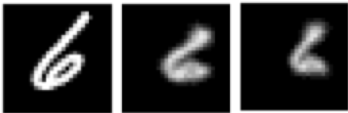
\includegraphics[width=0.4\columnwidth]{pic7.png}
}
\subfigure[] { \label{elastic1b}
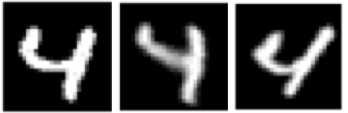
\includegraphics[width=0.4\columnwidth]{pic8.png}
}
\caption{\label{elast2}Two original hand written digit images, the number 6 (a) and the number 4 (b), each with two displacement maps (vertical and horizontal).}
\vspace{-10pt}
\end{figure}


%\textbf{Algorithm 1}
% If exists, Provide the pseudo code of your first algorithm behind this module
% Line-by-Line or block-by-block explanation for the pseudo code with reference to the line or the block in the algorithm.
% In this model, the input of each iteration is one batch of images with 28*28 pixels, whose value ranges from 0 to 255. The number of images in one batch is determined manually by a parameter in the implementation. In that training function, the input will go through the whole neural network model, including convolutional layers, sampling layers and common artificial layers. Neural network training process consists of forward propagation and backward propagation. Weights are updated and the offset calculated by the stochastic gradient descent method. The crucial idea here is one input is transmitted forward, processed by the convolutional kernel and the pooling kernel. 

% REMOVED THIS PARAGRAPH
%As a result, an output vector is given, whose maximum value indicates the prediction of the image character. Then backward propagation starts, and correctness of node weight is estimated by the error in one layer behind. All correctness, also called as offset of each node, are done based on the stochastic gradient descent method, and the update direction is indicated by the vectors discussed in the section \ref{subsec:problem}. One input picture in the batch would be analyzed and get a set of offsets. When all training samples are processed, the last step is to average output offsets as a final correction to the CNN model.

% \begin{algorithm}
% \caption{Naive CNN Training Algorithm}
% \label{alg1}
% \begin{algorithmic}
% \begin{codebox}
% \li $Get$ $path()$
% \li $Input \gets image$
% \li $Initialize$ $weights$
% \li $Training$ $Process$
% \li \For $each$ $training$ $iteration:$
% \li     \Do $Read$ $One$ $Batch$ $Input$
% \li         $Start$ $training$ $process :$
% \li         $Forward$ $propapagtion:$
% \li         \hspace*{1cm}$Convolution$ $process$
% \li         \hspace*{1cm}$Sampling$ $process$
% \li         \hspace*{1cm}$Fully$ $connected$ $process$
% \li         $Backward$ $propapagtion:$
% \li         \hspace*{1cm}$Calculate$ $gradient$ $descent$
% \li         \hspace*{1cm}$Weight$ $update$
% \li         $offset \gets backward$ $propagation()$ \End
% \li $Testing$ $Process$
% \li \For $each$ $testing$ $iteration:$
% \li     \Do $read$ $one$ $image$
% \li         $execute$ $CNN$ $model$
% \li 		$output \gets recognized$ $digit$
% \End
% \end{codebox}

% \end{algorithmic}
% \end{algorithm}



\subsection{Cost And Correctness Analysis}
\label{subsect:costanalysis}
Now we briefly describe the cost of the model. Originally, we assumed the training process of the naive CNN costs the time of $n$ and the testing process costs the time of $m$. Then in our model, we try to reduce the time consumption by distributed computing. If we use two process parallel computing, which means we assigns the input dataset into two different machines and do the training processes simultaneously, then theoretically the time cost of the training process in our model would be $n/2$. Moreover, if we assign the input dataset into $p$ different machines, then the training process costs $n/p$. Thus, in theory, the total time cost would be:
\begin{equation}
n/p+m
\end{equation}

However, we also need to consider the data communication between different machines in our project. Since in the combination step, we collect all the parameters in each model and calculate the final parameters, this part of time consumption is necessary. In our result we could see that the time cost of our model cannot reach the ideal situation, which is half of the original time consumption. 

% ======= END OF SECTION =======